\section{Macrobenchmarks}\label{sec:macrobenchmarks}
In order to not skew results towards \ac{JIT} compilers, because microbenchmarks are likely to be misleading \cite{sestoft2013microbenchmarks, microbenchmarkmislead}, we also implemented a macrobenchmark.
Some sources claim that \ac{JIT} provides speedup on loops, although according to a recent study this is not always the case \cite{vmwarmup}.

\subsection{Test Cases}
We defined a macrobenchmark as \dquote{\textit{a benchmark testing multiple units of functionality and excluding start-up time}}. As we have not been able to find any specific definition of macrobenchmarks in scientific literature, we decided to brainstorm some ideas. The ideas are as follows:
\begin{description}
    \item[Angry Physics] This test case is reminiscent of the game Angry Birds, hence the name. In this test a series of 3D objects (boxes, balls, pyramids, etc.) is placed on a platform. A canon that shoots is place at a distance from the platform. This canon will shoot projectiles of different size, mass and shape at the platform to trigger collisions and gravity simulation.
    \item[Wumpus World] In this case a 2D grid-based board is placed in the world. In the world an agent must collect a treasure and return to the start. The world is also inhabited by wumpuses, that wish to eat the agent. There are also a series of pits which the agent must avoid. The agent can sense wumpuses and pits on neighbouring grids by stenches and breezes respectively \cite{wumpus:world}.
    \item[Cowichan Problems] The Cowichan problems is a series of thirteen problems that mainly revolves around matrix and vector calculations \cite{wilson1995assessing}. The sizes of the matrices and vectors can be scaled to fit the size of the test and the problems chained to test different aspects of a language.
    \item[Game of Life] Game of Life is a cellular automaton described by John Conway \cite{game:of:life}. In the game organisms can be placed in a grid world. There are a series of rules, that determines how the organisms will evolve or die, that needs to be evaluated for each organism.
\end{description}

% Wumpus world: http://aima.cs.berkeley.edu/slides-pdf/chapter07-6pp.pdf
% Lund Universitet Applied Artificial Intelligence: http://cs.lth.se/edaf70/course-material/
We chose to implement the Wumpus World, as this macrobenchmark involves a set of classes including e.g. wumpus, world and agent. Furthermore, it is somewhat reminiscent of a game, being that it has an \ac{AI}-element along with the possibility of adding graphics. Even though it is a simulation of an \ac{AI} it has a deterministic behaviour on a given map.

\subsection{Rules in Wumpus World}
The Wumpus World is an N x M grid world. Each cell may contain one object. The Wumpus World uses the term \textit{neighbouring cells}. Given a cell X, it's neighbouring cells are that to the north, east, south or west of X. The cells on the diagonal are not considered neighbours. A visual representation, as presented in \cite{wumpus:world}, is shown in \figureref{wumpus:world}. A Wumpus can give off a stench so the agent know where the Wumpus could be, the same goes for for pits that have breezes next to it. Last there is Glitter which is the treasure, the agent wins when it gets back to start position (0,0), with the treasure.

\begin{figure}
    \centering
    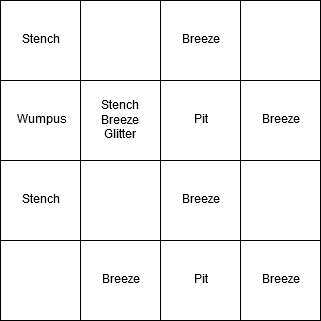
\includegraphics[width=.5\textwidth]{images/wumpus.png}
    \caption{A 4 x 4 Wumpus World with one Wumpus and two pits \cite{wumpus:world}}
    \label{fig:wumpus:world}
\end{figure}

An agent may take one of a couple of actions in each turn. They are as follows:
\begin{description}
    \item[Forward] The agent moves one step forward in its current direction.
    \item[Turn] The agent turns either left or right to change its direction.
    \item[Grab] The agent picks up the content of the current cell.
    \item[Release] The agent releases what ever it is holding and places it on the current grid cell.
    \item[Shoot] The agent shoots an arrow forwards from its current position to kill a wumpus in front of it.
    \item[Climb] The agent may climb out of the cave if it's located in the start position.
\end{description}

The agent is \dquote{blind} and may only perceive the world through percepts. The percepts are tied to objects, which are as follows:
\begin{description}
    \item[Agent] The agent is an \ac{AI}. It has a starting position and a goal of retrieving a treasure in the world. It must do so while minimising the score, i.e. the number of actions it has taken.
    \item[Wumpus] Wumpuses are hostile towards the agent. If the agent ends up in the same cell as a Wumpus, it will die. Wumpuses give of stench to the neighbouring cells. If the agent is sure of the location of a Wumpus, it may shoot to kill it (in which case the agent perceives a scream).
    \item[Pit] A pit is a hole in the ground. The agent will die if it falls into a pit and pits give of a breeze to neighbouring cells.
    \item[Treasure] There is one treasure in each map. The agent has the goal of getting to the treasure, picking it up and going back to the start state. A treasure gives off glitter to the cell it is placed in.
\end{description}
Apart from said percepts, the agent will perceive a bump if it walks into a wall.

\subsubsection{Simplifications}
In the implementation we make a couple of simplifications from the description in \cite{wumpus:world}. The first is that we abstract away the bump perception and instead assume that the agent knows its current position in the world.
The agent also knows where it has been, so it remembers its path.

Regarding the agent's actions several changes were made. We did so because the actions presented in \cite{wumpus:world} seemed a bit terse, most likely because they are meant to represent an actual robot. As a precise robot simulation is not desired in this case, we argue that the simplifications won't do any harm\todo{Meh. We should probably write something more scientific here.}. The actions were changed as follows:
\begin{description}
    \item[Grab and Release] The grab and release actions are replaced with a Boolean flag to indicate whether or not the agent has reached the cell that holds the gold. If the agent is in the start cell with the flag set to true, the map is completed.
    \item[Turn and Forward] The turn and forward actions are replace with a \ttt{Move(direction)}-action, that moves the agent in the given direction. Direction either being north, west, east or south.
    \item[Climb] Finally the Climb action was removed and instead a map is completed when the agent reaches back to the start cell or dies from walking into a pit or a wumpus.
\end{description}

\subsection{Platforms}
We chose Unity and Unreal for the test. Unity was chosen because it, according to statista.com in 2014, was used by 62\% of the responses in their survey \cite{gameengine:statista}.
Unreal was chosen because it was the fastest of all the engines in the microbenchmarks (see \secref{micro-benchmarking}).

\tmc{Write an explanation as to why we do not include a functional language}
%In this experiment we do not include a functional language, as we were not able to find a game engine with a functional language and Arcadia's res.

\subsection{Metrics}
Unlike the microbenchmarks that had a predefined metric of measuring time, macrobenchmarks does not. In order to formulate a baseline for the discussion on which metric to use, a series of questions were formulated:
\begin{itemize}
    \item How many worlds can we spawn at once while still producing at least 60 \ac{FPS}?
    \item How many turns can we execute per second?
    \item How much time does one tick take?
    \item What is the memory footprint per Wumpus World?
\end{itemize}
The first question is tied to the fact, that the macrobenchmark is run in a game engine. In the context of games it makes sense, as it is the metrics most often used by gamers. However, it make less sense if the macrobenchmark is not intended to test a game engine.

The second question is also directly related the behaviour of game engines, but is disconnected somewhat from the user experience. Instead this is a measure of the raw computational throughput. \todo{This is thin.}

The third question has the advantage, that it pairs well with the metrics used in the microbenchmarks and the fourth, that memory is also a performance concern, that we have only briefly discussed previously in this project.

We choose to examine the last two questions by reusing the timer code that was written for the microbenchmarks along with examining memory use per instance of the wumpus world. The timing code was use to measure how long time each invocation of the \ttt{World}'s \ttt{Iterate}-method took. The \ttt{Iterate}-method is responsible for all Wumpus World-related logic, such as generating percepts for the agent, updating the agent's perceived world state etc. The test would run until the agent found the treasure and made it back to its start position. This was repeated 10 times for the same map. 

In performance benchmarking memory is naturally also of great concern, however, we could not find a meaningful way of measuring memory usage in Unreal Engine at the time of writing. Unreal Engine has a profiler tool that can measure the time it takes to generate a frame, but it's memory section is currently work-in-progress \cite{unreal:profiler}. The current state of the profiler plots a graph with frame count along the Y-axis and time along the X-axis. It provides an overview of all memory consumption in the game, but when they are plotted on the graph, they are so using frame count and time. Furthermore, it was not possible to plot one single graph over all memory consumption, but only for each component (of which there are around 200 in the profiler tool). Left with the option of examining Unity's memory without possibilities for comparison, we decided that memory benchmarking be left as future work.

\subsection{Results}
The results from the macrobenchmark is plotted in \figureref{macro-results}. The spikes in Unreal Engine's performance (iteration 14, 28 etc.) correspond to clearing the agent's state and beginning the next iteration. In the case of Unity, the execution time for the agent's first tour through the map is much higher than that of Unreal Engine. The execution time in Unity stabilises in the third iteration, approaching Unreal Engine's performance. Interestingly, the spikes that correspond to starting over are higher in Unreal Engine than they are in Unity. This comes at the cost of Unity's execution time spiking when not clearing the map, which could be caused by garbage collection. Generally Unreal Engine's execution times are more stable and predictable than those of Unity.

\begin{figure}
    \centering
    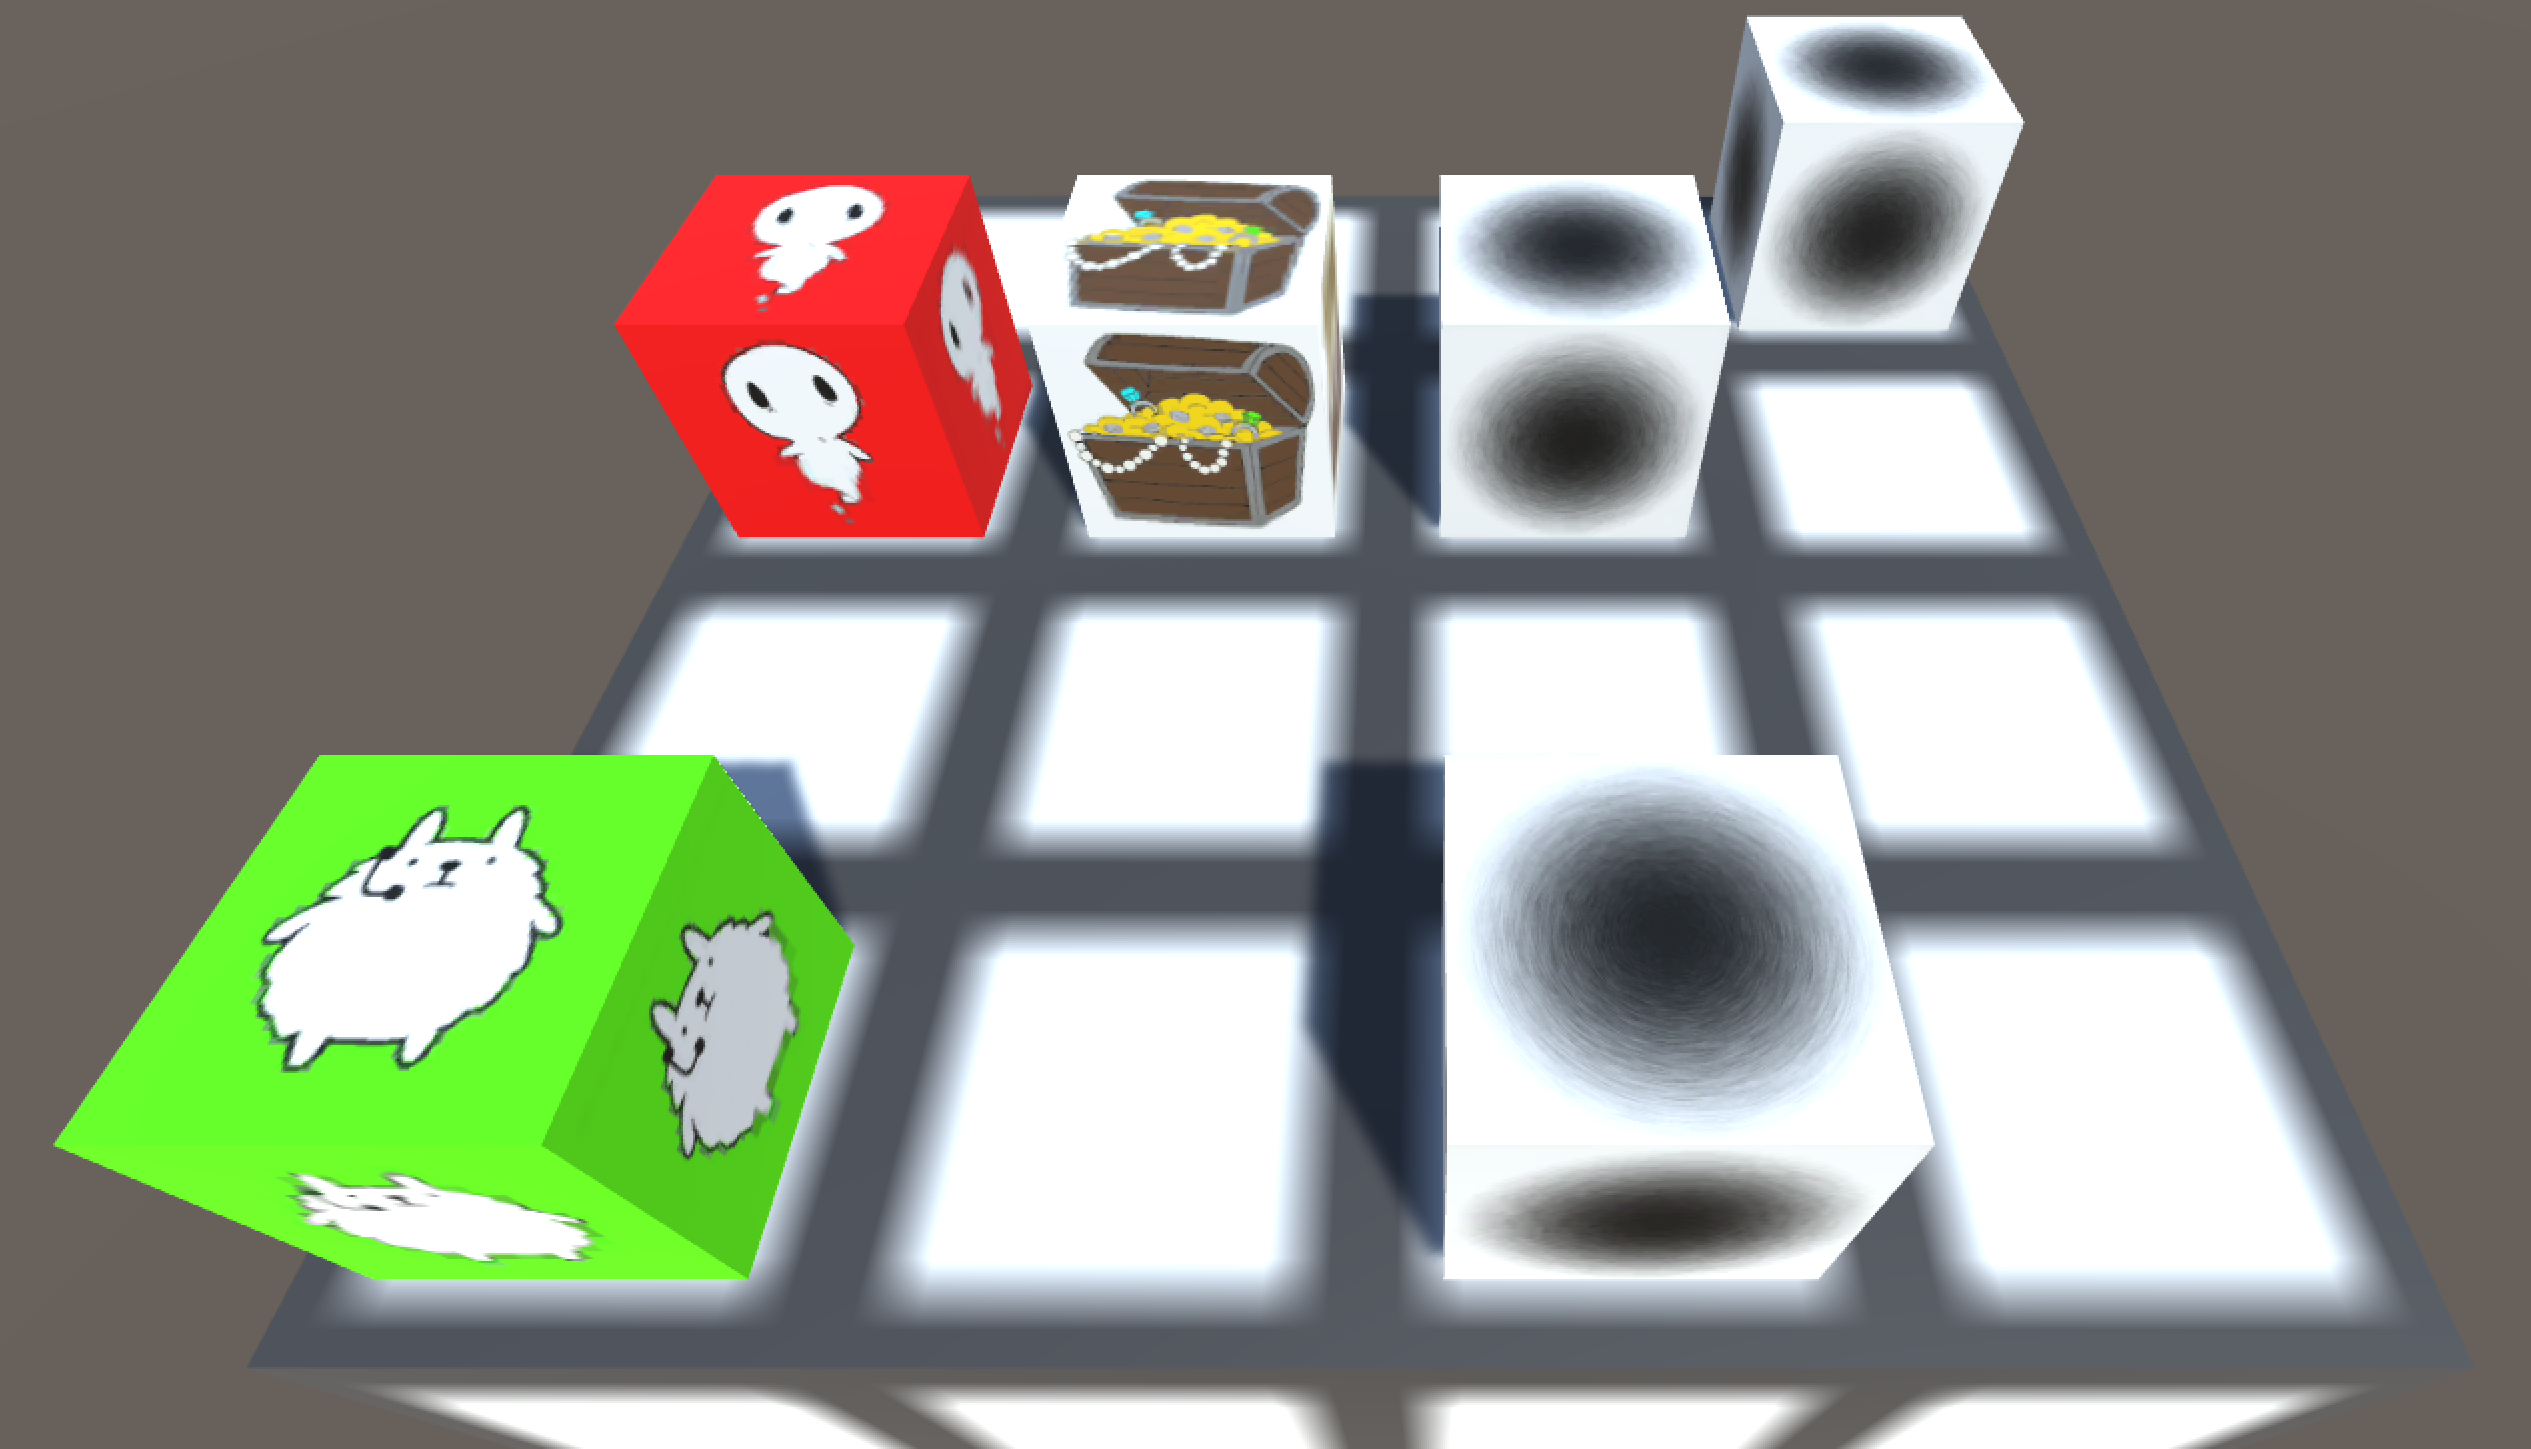
\includegraphics[width=\textwidth]{images/Wumpus_Unity.png}
    \caption{Wumpus implementation in Unity, the map is the same as in \figureref{wumpus:world}}
    \label{fig:wumpus:world:unity}
\end{figure}

\begin{figure}[H]
    \makebox[\textwidth][c]{
    \begin{tikzpicture}
    \tikzset{every mark/.append style={scale=.5}}
        \begin{axis}[
                width=1.25\textwidth, 
                height= 8cm,
                ylabel={Run time in microseconds},
                xlabel={Iteration No.},
                ymin = 0,
                ymax = 1500,
                xmin = 0,
                xmax = 130,
                ymajorgrids,
                legend columns = -1,
                area legend,
                legend style={draw=none,at={(0.5,1.05)},anchor=south, column sep=1ex}
            ]
            \addplot[mark=*, color=red] table [x={Iteration No.}, y=Unreal] {\macroData};
            \addplot[mark=*, color=blue] table [x={Iteration No.}, y=Unity] {\macroData};
            \legend{Unreal, Unity}
        \end{axis}
    \end{tikzpicture}}
    \caption{Wall clock-time for each invocation of the \ttt{World.Iterate}-method}
    \label{fig:macro-results}
\end{figure}